\section{Affine reconstruction}

\begin{theorem}
    A projective transformation $\mathbf{H}$ that maps the line at infinity $\mathbf{l}_{\infty}$ onto itself implies that $\mathbf{H}$ is affine.
\end{theorem}
\begin{proof}
    A point at infinity, represented as $\mathbf{x}_{\infty}=\begin{bmatrix} x & y & 0 \end{bmatrix}^T$, is mapped to another point $\mathbf{x}^\prime=\mathbf{Hx}_{\infty}$ to remain a point at infinity, its third coordinate must be zero. 
    This condition can be expressed as:
    \[\begin{bmatrix} v_1 & v_2 & 1 \end{bmatrix} \begin{bmatrix} x \\ y \\ 0 \end{bmatrix}=0 \]    
    Which simplifies to:
    \[\begin{bmatrix} v_1 & v_2 & 1 \end{bmatrix} = \begin{bmatrix} 0 & 0 & 1 \end{bmatrix}\]
    Thus, the matrix $\mathbf{H}$ has the structure of an affine transformation, confirming that $\mathbf{H}$ is affine.
\end{proof}
In an image produced by a general projective transformation of a scene, the line at infinity $\mathbf{l}^\prime_{\infty}$ in the image will not coincide with the original line at infinity $\mathbf{l}_{\infty}$. 
However, this difference can be exploited by using $\mathbf{l}^\prime_{\infty}$ as additional information.
By applying a corrective projective transformation $\mathbf{H}_{\text{AR}}$ that maps $\mathbf{l}^\prime_{\infty}$ back to $\mathbf{l}_{\infty}$, a modified image is obtained.
In this new image, the line at infinity $\mathbf{l}_{\infty}$ is preserved.

According to the theorem, this resulting transformation produces a model that is an affine mapping of the original scene. 
Therefore, the modified image is an affine reconstruction of the scene.
\begin{figure}[H]
    \centering
    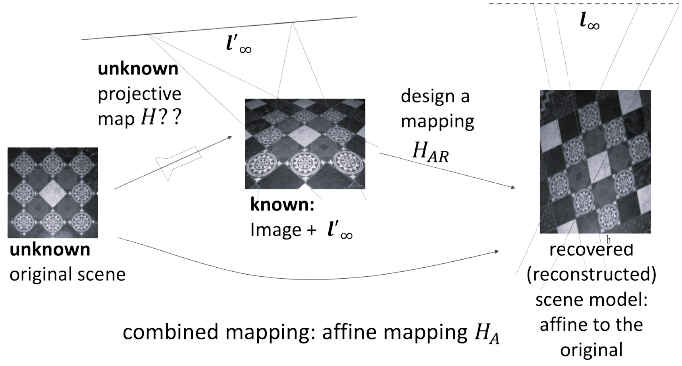
\includegraphics[width=0.75\linewidth]{images/HAR.png}
    \caption{Affine transformation}
\end{figure}
The key challenges in this approach are:
\begin{itemize}
    \item Determining the projective transformation $\mathbf{H}_{\text{AR}}$ that maps $\mathbf{l}^\prime_{\infty}$ back to $\mathbf{l}_{\infty}$.
    \item Identifying the vanishing line in the image, which corresponds to $\mathbf{l}^\prime_{\infty}$.
\end{itemize}

\subsection{Projective transformation determination}
o find the corrective projective transformation $\mathbf{H}_{\text{AR}}$ that restores $\mathbf{l}^\prime_{\infty}$ to $\mathbf{l}_{\infty}$, the mapping must satisfy the condition that any point $\mathbf{x}^\prime \in \mathbf{l}^\prime_{\infty}$ is mapped to a point at infinity.
Mathematically, this can be written as:
\[\mathbf{H}_{\text{AR}}\mathbf{x}^\prime = \begin{bmatrix} * \\ * \\ 0 \end{bmatrix}\]
The transformation $\mathbf{H}_{\text{AR}}$ can be represented in matrix form as:
\[\mathbf{H}_{\text{AR}} = \begin{bmatrix} * & * & * \\ * & * & * \\ & \mathbf{l}^{\prime T}_{\infty} & \end{bmatrix}\]
which ensures that any point $\mathbf{x}^\prime \in \mathbf{l}^\prime_{\infty}$ is correctly mapped to the line at infinity.

\subsection{Vanishing line identification}
To identify the vanishing line $\mathbf{l}^\prime_{\infty}$, additional geometric information can be used, such as the images of parallel lines in the scene. 
These parallel lines intersect at points on the vanishing line in the projective image.
\begin{figure}[H]
    \centering
    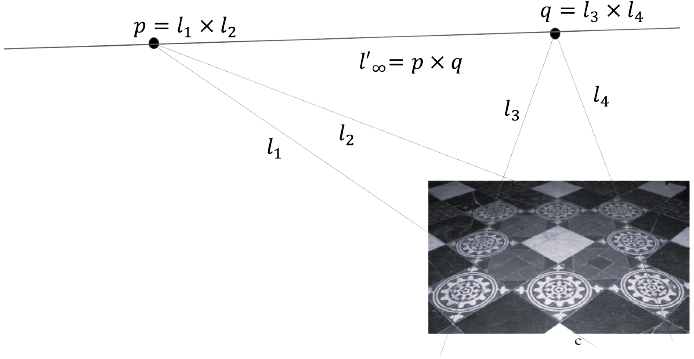
\includegraphics[width=0.5\linewidth]{images/van.png}
\end{figure}
By leveraging such information, the vanishing line can be accurately determined, enabling the projective transformation $\mathbf{H}_{\text{AR}}$ to be applied for an affine reconstruction of the scene.